\section{Experiment}
During the first part of the lab, we measured the intensity of a white diode at different voltages. The white diode was a violet diode, covered in a phosphorus layer that emitted a white spectrum. The voltage was controlled through a DC source, as shown in \autoref{fig:part1_circuit}. Twelve measurements were taken of the voltage from the DC source, the voltage across the diode, the current through the circuit, and the intensity. The measurements were taken evenly between 1 to \SI{9}{\volt}. The input voltage had an accuracy of two significant figures, while the voltmeter and ammeter had an accuracy of three significant figures. However, the error in these measurements was not accounted for. 

The intensity of the diode was evaluated through an glass fibre cable placed directly above the diode. The intensity was displayed in a computer program called AvaSoft, where counts for different wavelengths were shown. The intensity was determined by evaluating the intensity at the largest peak. The integration time used was \SI{70}{\milli\s}, which involved averaging every 10th measurement. This measurement involved values with two decimal places and significant figures ranging from three to seven. However, the actual accuracy is likely much lower due to the influence of other light sources in the room.

In the second part, the same circuit was used; however, this time a yellow diode was employed instead. The fibre optic cable was taped directly onto the diode. One measurement was taken of the voltage from the DC source, the voltage across the diode, the current through the circuit, and the intensity. A screenshot was also captured of the spectrum in the AvaSoft program. Keeping the same voltage from the DC source, the diode was placed in liquid nitrogen, and a similar measurement was taken.

In the last part, another circuit was used, as seen in \autoref{fig:part3_circuit}. This time, neither an ammeter nor a voltmeter was used in the main circuit. Instead, a separate circuit was implemented with a diode and a voltmeter connected in parallel. The integration time was changed to \SI{2}{\milli\s}. The DC source was turned on until the diode in the main circuit shone brightly. The other circuit was then placed close to the main circuit to check if the diode in the smaller circuit registered any voltage. This procedure was repeated for all combinations of red, green, and blue diodes.



\begin{figure}[H]
    \centering
    \begin{subfigure}{0.3\textwidth}
        \centering
        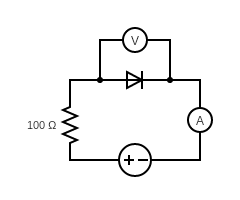
\includegraphics[width=\textwidth]{Figures/circuit_part1.png}
        \subcaption{This sktch shows the circuit for part 1 and part 2. }
        \label{fig:part1_circuit}
    \end{subfigure}
    \hspace{2cm}
    \begin{subfigure}{0.3\textwidth}
        \centering
        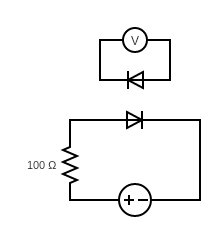
\includegraphics[width=\textwidth]{Figures/circuit_part3.png}
        \subcaption{This sktch shows the circuit for part 3, with the two different diodes. }
        \label{fig:part3_circuit}
    \end{subfigure}
    \caption{Above one can see the circuits used in this lab. Both circuits used an resistor with \SI{100}{\ohm} and a DC-source. }
    \label{fig:circuits}
\end{figure}
